\section{Experiments}

\subsection{BranchyNet}

BranchyNet \cite{teerapittayanon_branchynet:_2016} proposed by \citeauthor{teerapittayanon_branchynet:_2016} is an early exiting framework for fast inference of a \gls{dnn}. The work states, that typically samples can be accurately classified using less \gls{dnn} layers which can improve the inference time, if a sample cannot be classified with proper confidence more layers can be used to obtain a more confident prediction. The framework show promising results of reduced inference time, added regularization via joint optimization of exiting points and mitigation of vanishing gradients. The result are based on three well-known \gls{dnn} architectures; LeNet \cite{bibid}, AlexNet \cite{bibid} and ResNet \cite{he_deep_2015}, modified to implement the BranchyNet framework, and to accommodate the MNIST \cite{bibid} and Cifar-10 \cite{bibid} datasets. 

One may argue, that the two datasets used for benchmarking are not applicable to real-life scenarios, as the images are only 32x32 pixels and the datasets only contain 10.000 samples.

This thesis studies BranchyNet on state-of-the-art \gls{dnn} ResNet50 fo image size 224x224 images, only modified to accommodate early exiting of the BranchyNet framework. ResNet50 is built up of 50 layers divided into 4 blocks, these blocks are decided to be the initial exiting points. After each block, the intermediate features are fed to a pooling-layer and a fully-connected classifier. The prediction results are stored and the networks intermediate features are further processed until the end of the original network.

\begin{figure}
	*Figure of B-ResNet50*
	\caption[B-ResNet architecture]{ResNet50 extended to implement the BranchyNet framework.}
	\label{b-resnet}
\end{figure}

The network is trained solving the joint-optimization problem is defined as the weighted sum of each branch-prediction.

\begin{align*}
	L(\hat{\mathbf{y}},\mathbf{y};\theta) = \sum_{n=1}^{N} w_m L(\hat{\mathbf{y}}_{exit_n},\mathbf{y};\theta)
\end{align*}

Where the loss function is the softmax cross-entropy objective.
The weighted sum loss is back-propagated to optimize the weights of the network. 

\subsubsection{Training BranchyResNet}

The B-ResNet is trained on the *-dataset \cite{dataset}. The model is trained on a single \gls{gpu} GTX1080 with 12Gb memory. Typically a batch size of 32 is chosen, however smaller batch size, have shown better generalization performance \cite{masters_revisiting_nodate}, thus a batch size of 16 is chosen, which also is maximum to prevent memory exhaustion and still have descent training times. The network weights are initialized as pre-trained ImageNet \cite{deng_imagenet:_2009}, to reduce model convergence time and improve model accuracy \cite{yosinski_how_2014}. The network classifiers are rough-tuned by freezing the model feature extractor for X epoch with a learning rate of Y. The entire network is then made trainable and trained for Z epochs.

\begin{figure}
	
	\centering
	\captionsetup[subfigure]{justification=centering}
	\subfloat[Train loss\label{fig:B-resnet-voc-train-loss}]{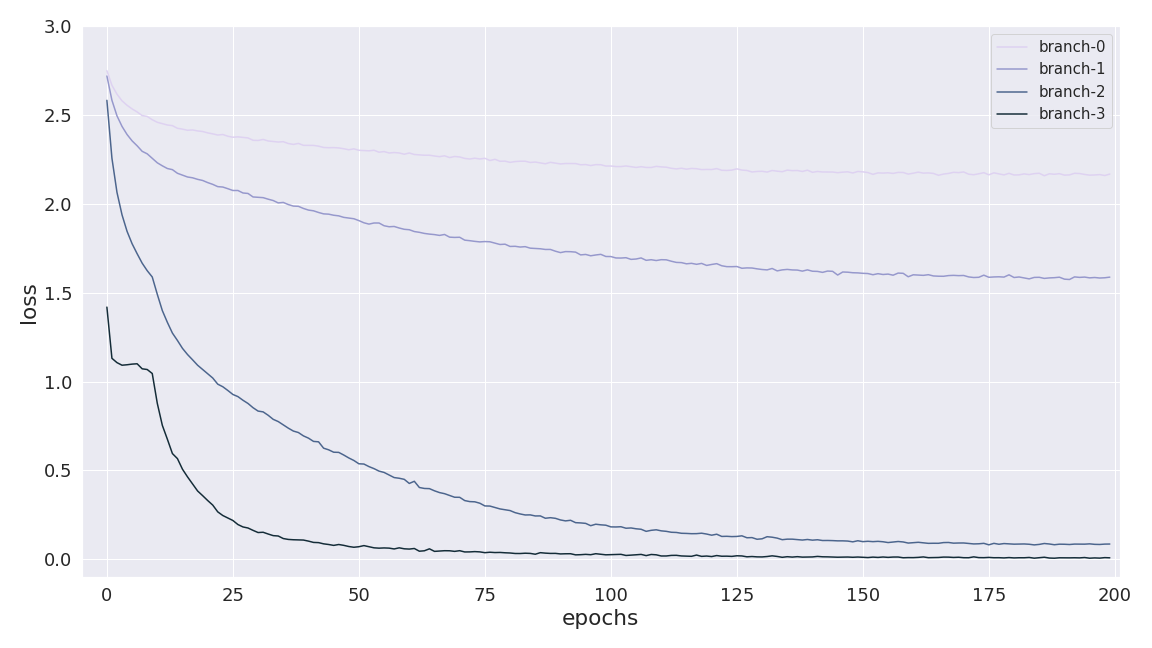
\includegraphics[width=.49\textwidth]{figures/BResNetVOC/BResNet_train_loss_VOC.png}}
	\subfloat[Test loss \label{fig:B-resnet-voc-test-loss}]{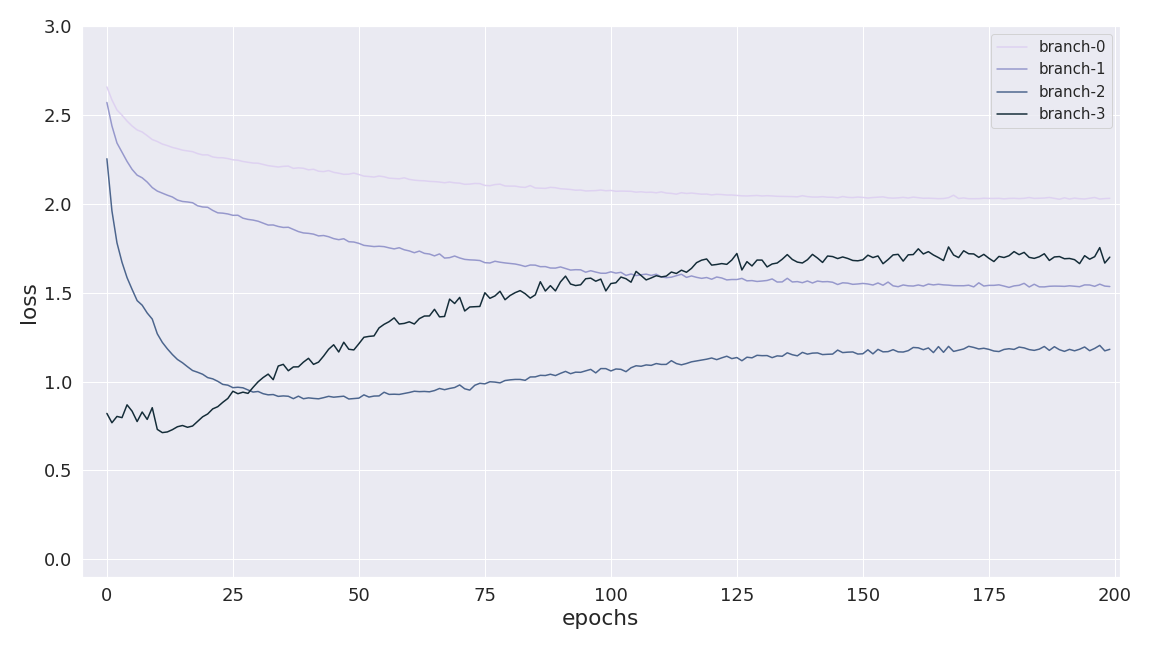
\includegraphics[width=.49\textwidth]{figures/BResNetVOC/BResNet_test_loss_VOC.png}}
	\hfill
	\subfloat[Train accuracy\label{fig:B-resnet-voc-train-acc}]{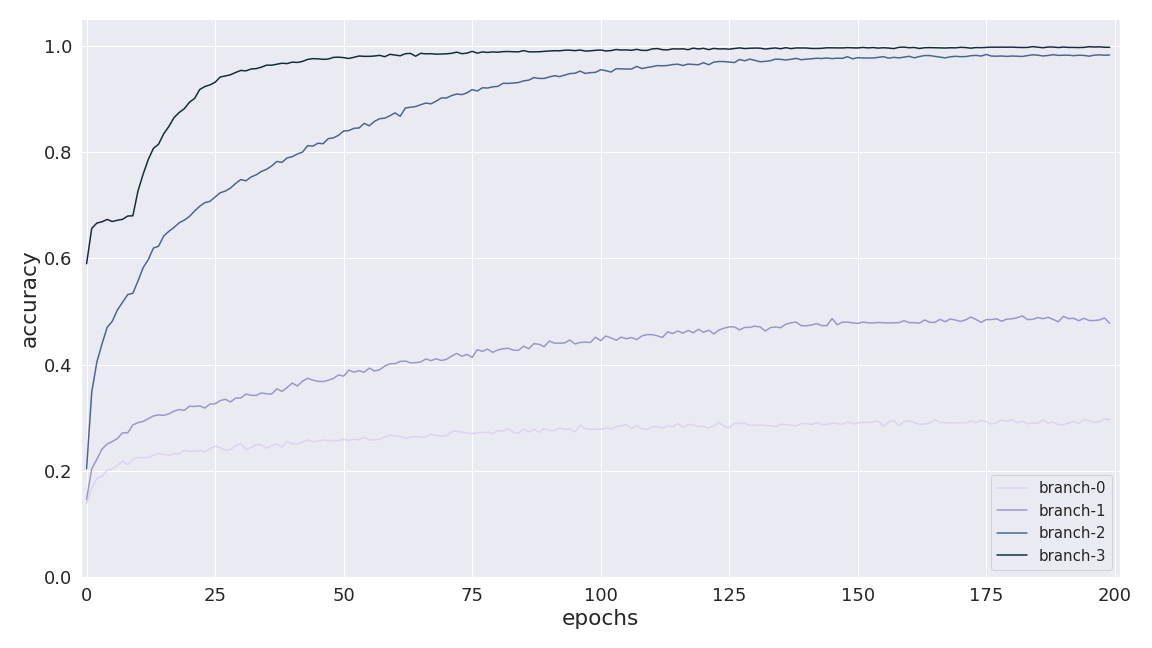
\includegraphics[width=.49\textwidth]{figures/BResNetVOC/BResNet_train_acc_VOC.png}}
	\subfloat[Test accuracy\label{fig:B-resnet-voc-test-acc}]{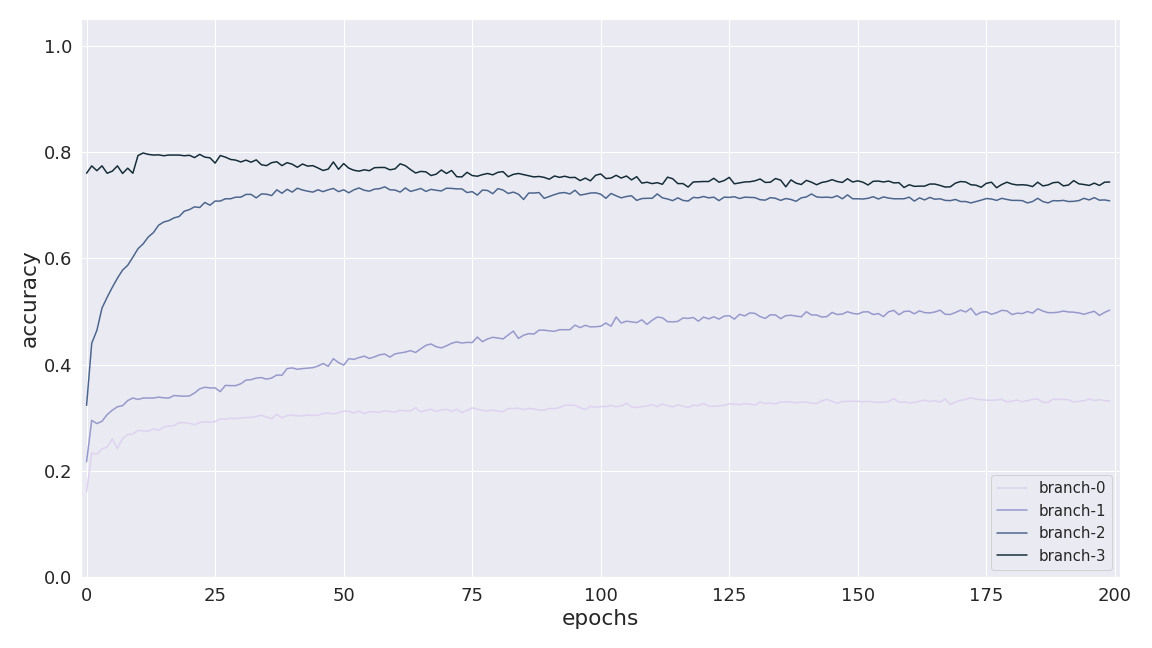
\includegraphics[width=.49\textwidth]{figures/BResNetVOC/BResNet_test_acc_VOC.png}}
	\caption[B-ResNet VOC Training summary]{Training summary shows the progression of model attributes over times of epochs, \protect\subref{fig:B-resnet-voc-train-loss} train loss, \protect\subref{fig:B-resnet-voc-test-loss} test loss, \protect\subref{fig:B-resnet-voc-train-acc} train accuracy, \protect\subref{fig:B-resnet-voc-test-acc}, test accuracy.}
\end{figure}

Visualizing the training progression, clearly indicates that model overfitting to the training data. When a model overfits it suffers to generalize the true underlying distribution of the data. This can be caused by insufficient number of training samples or too complex a model. Since the model has shown promising results in image classification task previously, we can conclude, that the dataset is too sparse.

Even though the model fails to generalize, the experiment still produce interesting results. Given an early exiting model as B-ResNet 50\% of the test samples can be correctly classified using only half of the \gls{dnn}.

\subsection{\acrlong{ddnn}}

\gls{ddnn} \cite{teerapittayanon_distributed_2017} also proposed by \citeauthor{teerapittayanon_distributed_2017}, extend upon early exiting models and model partitioning,  to  create a distributed computing hierarchy over cloud, edge and end devices. The idea is having the same shallow model running on multiple end-device, that collaboratively classifies the object. If the network of end devices cannot obtain a classification of satisfactory confidence, a larger model taking the output features from all end-devices as input, is run on a \gls{lan} connected edge server. 

\begin{figure}
	*Figure of DDNN-ResNet50*
	\caption[\gls{ddnn}-ResNet architecture]{ResNet50 extended to implement the \gls{ddnn} framework.}
	\label{ddnn-resnet}
\end{figure}

The distributed network is trained solving the same joint-optimization problem as for BranchyNet.

\begin{align*}
L(\hat{\mathbf{y}},\mathbf{y};\theta) = \sum_{n=1}^{N} w_m L(\hat{\mathbf{y}}_{exit_n},\mathbf{y};\theta)
\end{align*}

Where the loss function is the softmax cross-entropy objective.
The weighted sum loss is back-propagated to optimize the weights of the network. 

Being a distributed system comes with all the fallacies and benefits from distributed computing e.g. fault tolerance etc.

\subsubsection{Training \gls{ddnn}}

\subsection{Transport Protocol} 

Offloading tasks over the network, irregardless fully or partially requires a transport protocol. The selection is typically a choice of either \gls{tcp} or \gls{udp}. \gls{tcp} is a reliable protocol, that guarantee no losses by retransmission of lost packets. \gls{udp} on the other hand is a best-effort protocol, that accept packets loss, thus not introducing any communication overhead such as retransmissions. 


Fully offloading \gls{jpeg} compressed images for classification require no losses for human-readability. Sending intermediate features of a \gls{dnn} may not be as intolerant to losses and might be able to function with the far more lightweight \gls{udp}. In current research literature the choice of \gls{tcp} seems given in advance.  


In this experiment the \gls{tcp} transmission time and retransmission rate is investigated under different communication environments. 